\chapter{Experimental Results} % (fold)
\label{cha:experiments}

This chapter presents the experimental work completed to validate the actuator dynamics and motion control framework used in simulation. It is important to test walking control strategies on physical hardware directly due to the imperfections in a simulation environment. For example, the contact models used to estimate the ground reaction force is only an approximation. There are also other unmodeled effects which can significantly alter the dynamics of the physical system (i.e. vibrations). The simulations used to demonstrate the proposed 3D FPE walking control strategy in the previous section was designed to account for link side dynamics only. Section~\ref{sec:actuator_model} describes the modifications to account for the actuator dynamics. This modification to the simulations enables a single controller designed in Simulink to target either the simulation environment or the physical hardware using the HIL architecture discussed in Section~\ref{sec:hil_architecture}. The experimental validation for a single actuator and the proposed motion control framework are presented in Sections \ref{sec:1dof_validation} and \ref{sec:motion_control_validation}, respectively. 

\section{Actuator Model} % (fold)
\label{sec:actuator_model}
In the ideal case, the control signal $\vec{u}$ applied to each joint would simply be $\vtau$ shown on the right hand side of (\ref{eq:eom1}). However, 

\begin{figure}[!h]
	\centering
    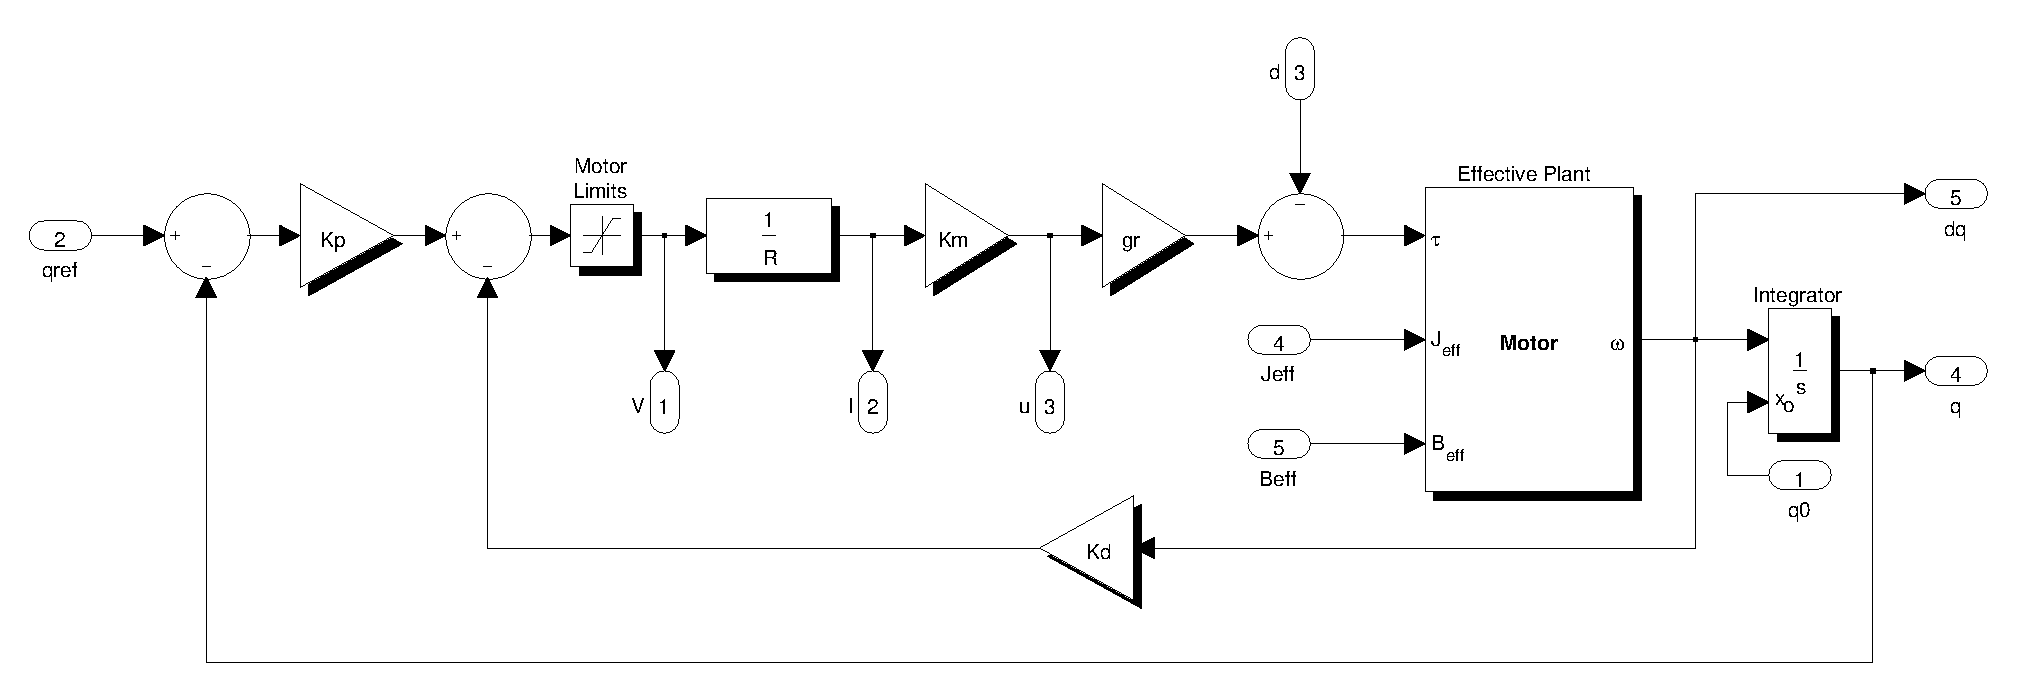
\includegraphics[scale=0.5]{fig/experiments/pdmotorcontroller.eps} 
  	\caption{PD Controller implementation for independent joint control with actuator dynamics.}
	\label{fig:pdmotorcontroller}
\end{figure}

% section actuator_model (end)

\section{HIL Architecture} % (fold)
\label{sec:hil_architecture}
Incomplete. 

\begin{figure}[!h]
	\centering
    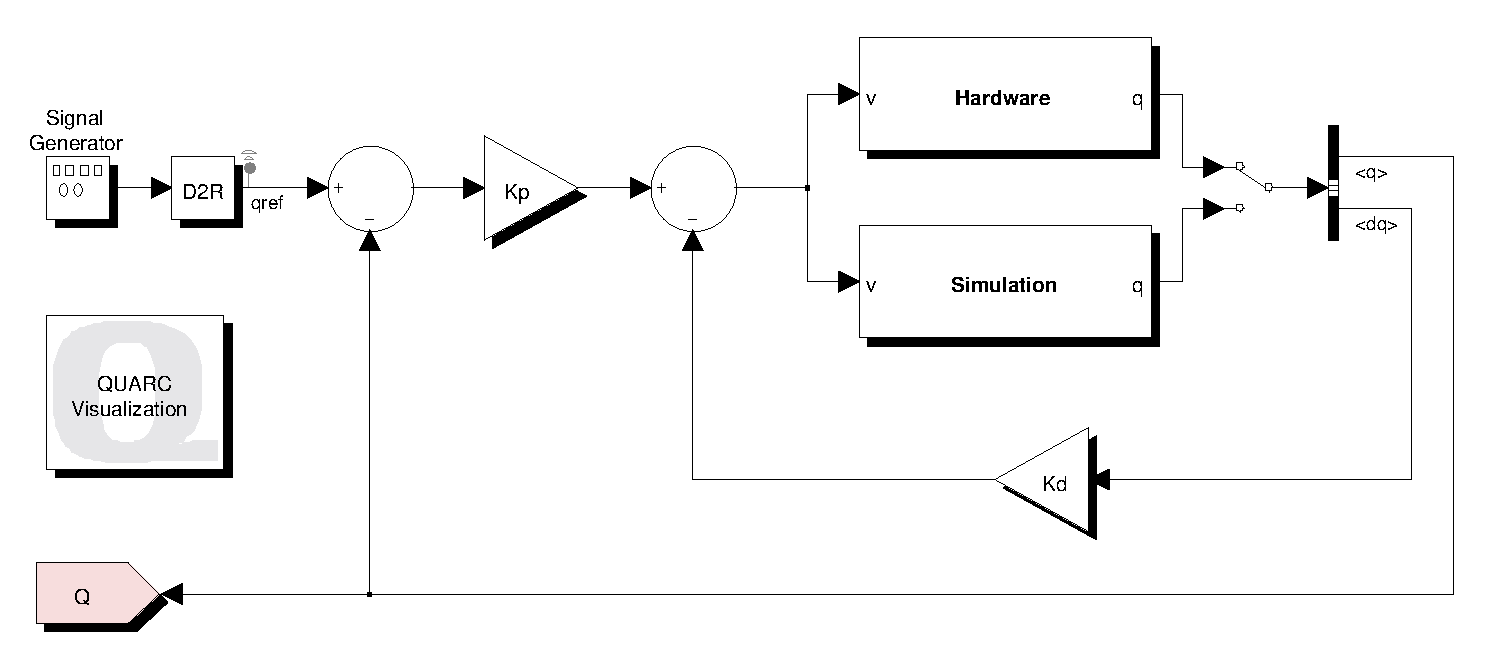
\includegraphics[scale=0.6]{fig/experiments/parallelmodels.eps} 
  	\caption{Parallel models designed to target either simulations or physical hardware with the same controller.}
	\label{fig:parallelmodels}
\end{figure}

\begin{figure}[!h]
	\centering
    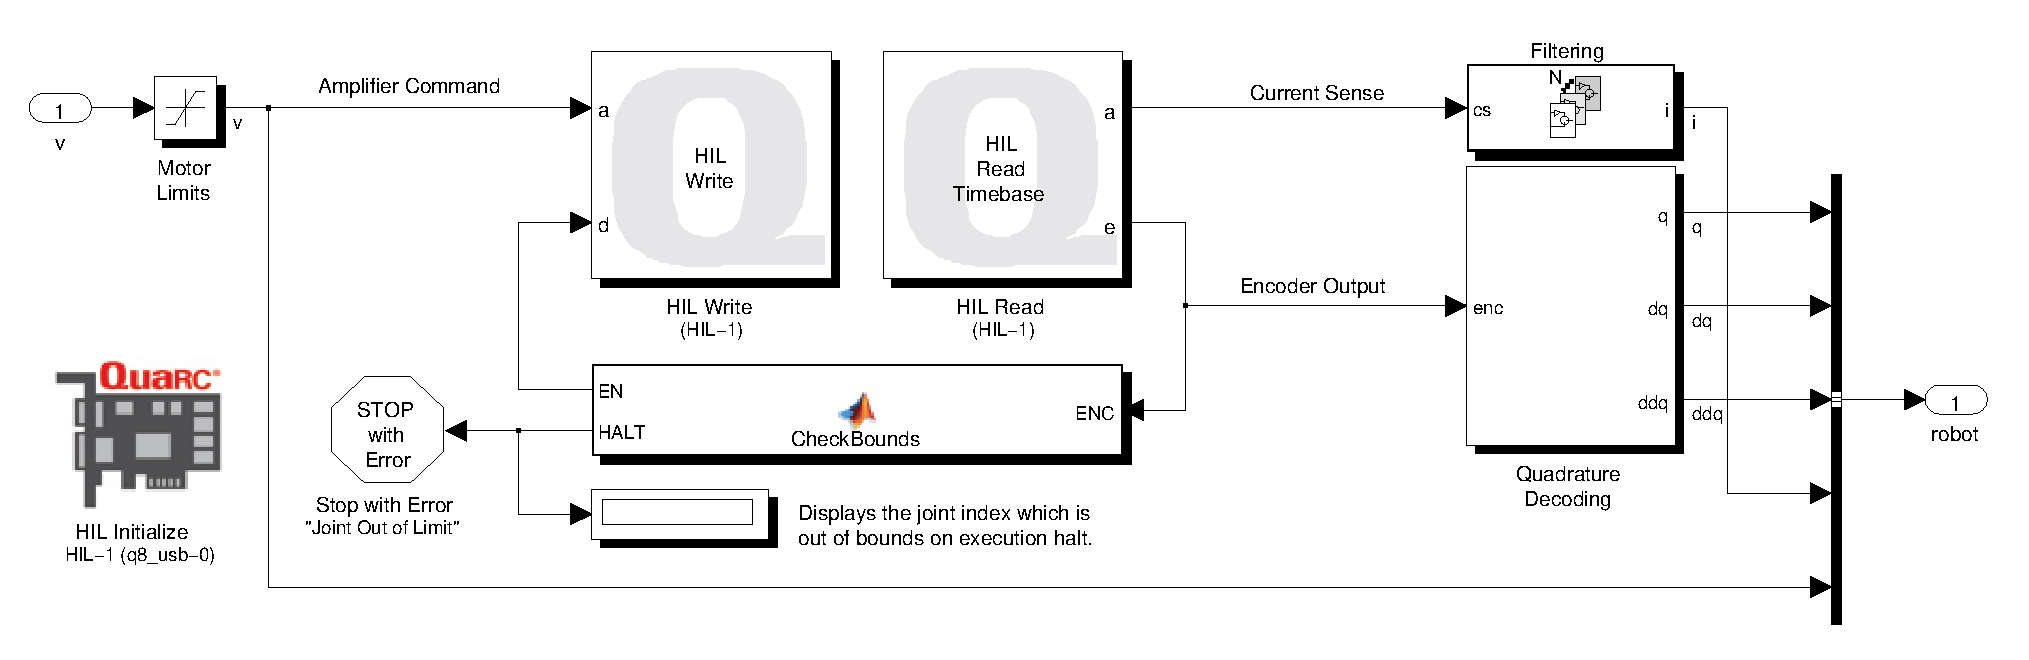
\includegraphics[scale=0.45]{fig/experiments/hilmodel.eps} 
  	\caption{HIL subsystem from Figure~\ref{fig:parallelmodels} used to target physical hardware with voltage control signal.}
	\label{fig:hilmodel}
\end{figure}

\begin{figure}[!h]
	\centering
    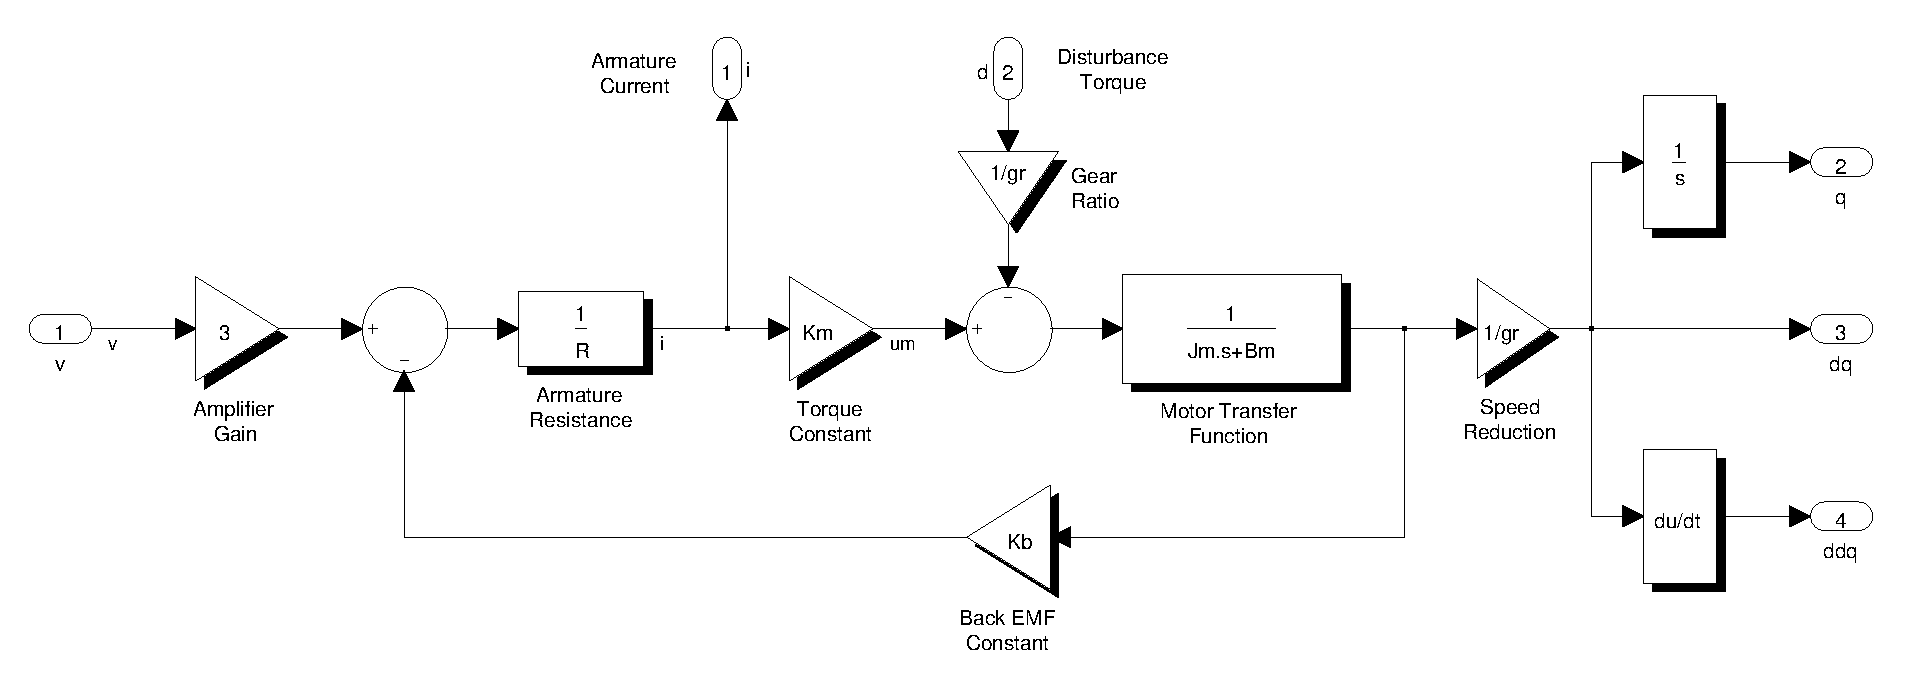
\includegraphics[scale=0.55]{fig/experiments/simmodel.eps} 
  	\caption{Subsystem from Figure~\ref{fig:parallelmodels} used to target the simulated environment with voltage control signal.}
	\label{fig:simmodel}
\end{figure}

% section hil_architecture (end)

\section{Single DOF Validation} % (fold)
\label{sec:1dof_validation}
Incomplete. 
% section 1dof_results (end)

\section{Motion Control Validation} % (fold)
\label{sec:motion_control_validation}
\Incomplete. 
% section motion_control_results (end)

\section{Discussion} % (fold)
\label{sec:experiments_discussion}
Incomplete. 
% section discussion (end)

% chapter experiments (end)